% Online Software Overview

The pixel online software is based on the xdaq toolkit and is
built from a number of different components (applications). The
different xdaq based components are shown in green in 
Fig.~\ref{fig:components}. The top level application is the 
PixelSupervisor. This application is responsible for the overall
coordination of the pixel DAQ. The PixelSupervisor talks to the
supervisors that directly control the hardware. For example 
we have the PixelFECSupervisor that provides the interface to the
pixel FECs. Similarly the PixelFEDSupervisor controls FEDs. 
In production at P5, there are multiple instances of the PixelFECSupervisor and
PixelFEDSupervisor; one per VME crate.\footnote{The strip tracker
uses a design where there is one supervisor per VME board.}

The PixelTKFECSupervisor controls the tracker FEC hardware. The
pixel system uses the tracker FEC hardware slow I2C to
initialize the fast I2C used for the download of most 
configuration data.

The PixelTTCSupervisor controls the pixel TTC module used for trigger
and timing. Among other things the TTC module is used during
calibrations to generate triggers. In modern releases of the software,
the PixelTTCSupervisor has been deprecated in favor of the
TTCciControl, which is a standard package maintained by the TTC group.

The PixelLTCSupervisor is used for the local trigger control.

The various supervisors run as indepdendent processes, or even on
different computers. Therefore, in order to communicate with each
other they must exchange messages on the network. This is done using
the SOAP protocol.

The Level 1 function manager (L1FM or FM) for the pixels is the
interface the pixel system has to the global run control (RCMS for
Run Control and Monitoring System). The FM is a java application.
It responds to requests from RCMS to change states in the 
state diagram that describe the state of the DAQ system. This
state diagram is shown in Fig.~\ref{fig:l1fm}.  The pixel
FM is a relatively thin layer that basically just passes the state
changes on to the PixelSupervisor. 

\begin{figure}
\begin{center}
 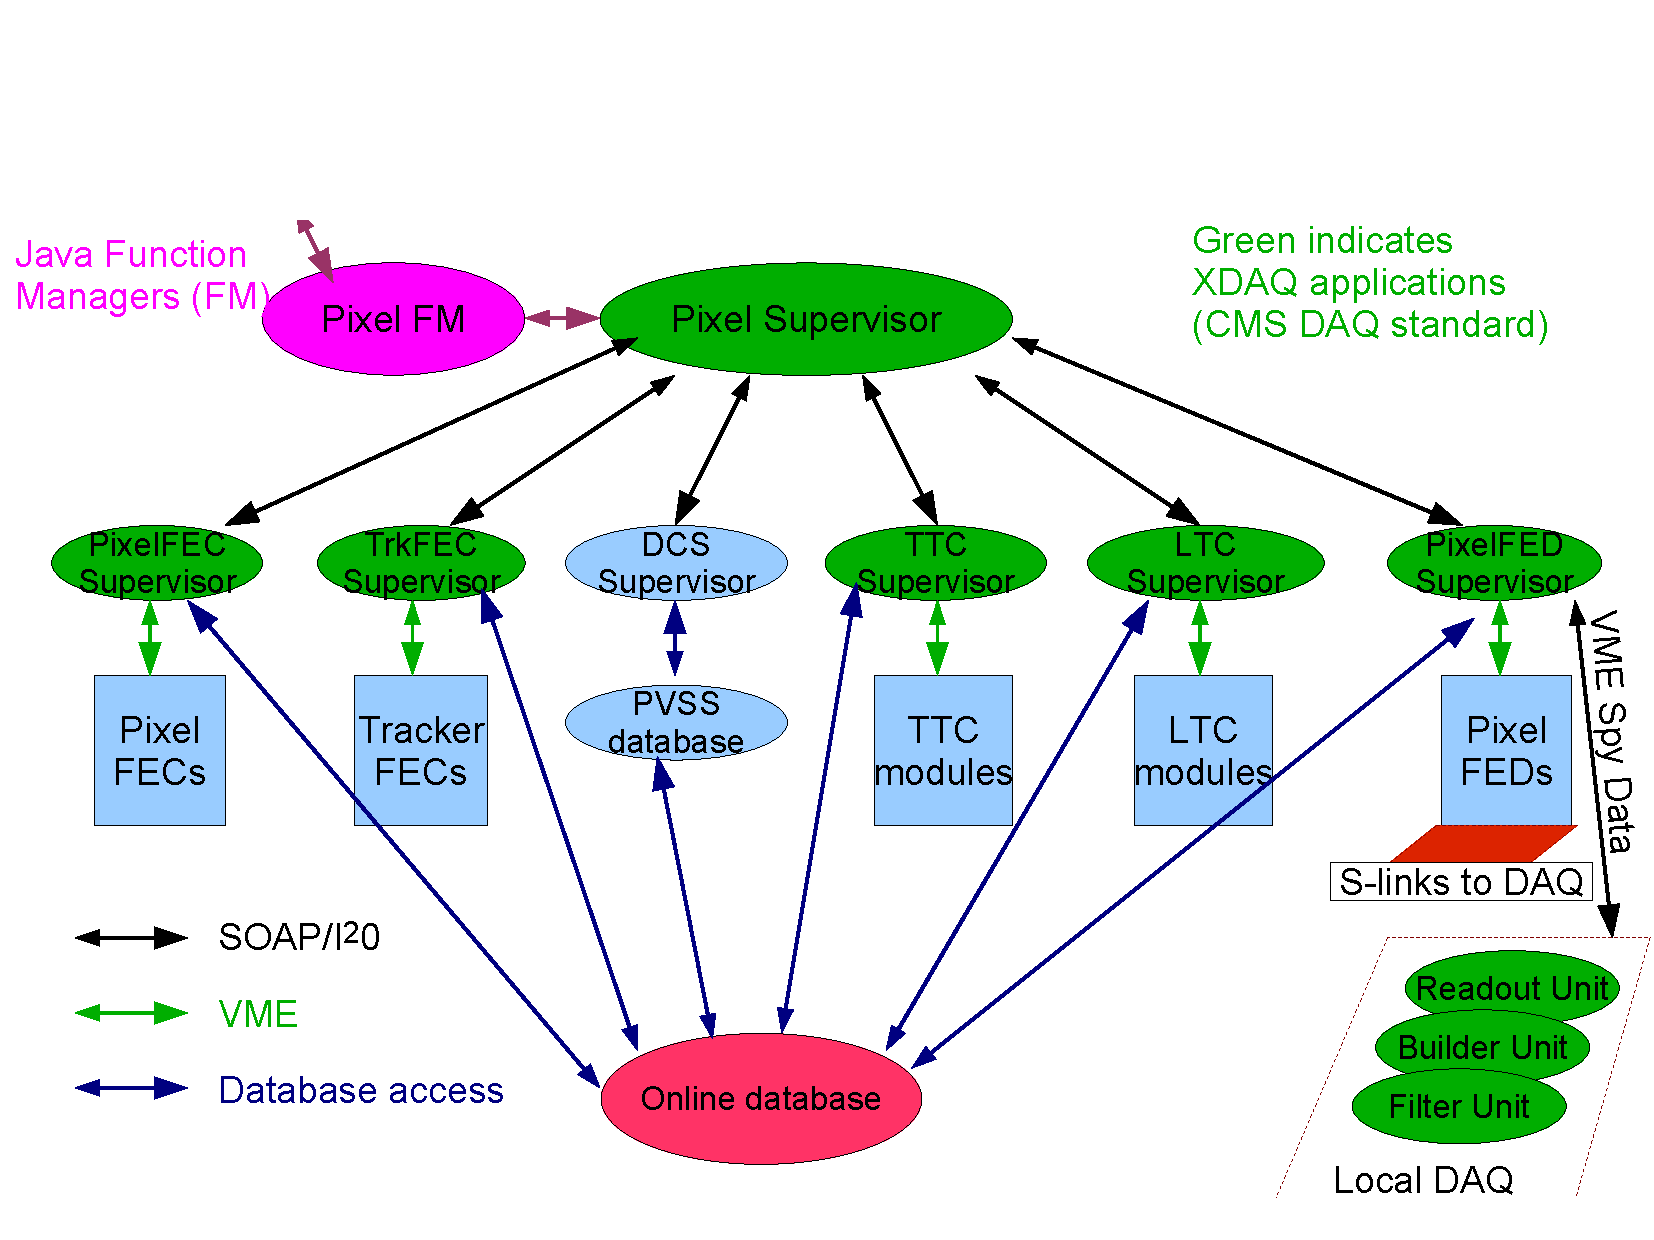
\includegraphics[width=0.99\textwidth]{POScomponents.pdf}
\end{center}
\caption{The different applications that compose the Pixel Online Software.}
\label{fig:components}
\end{figure}

